\documentclass[12pt]{article}
\usepackage[tmargin=1.25in,lmargin=.75in,rmargin=1in,bmargin=1in,paper=letterpaper]{geometry}
\usepackage{amsmath,amssymb, amsfonts}
\usepackage{multirow, color}
\usepackage{mathrsfs} % for \mathscr{S}
\usepackage{fancyhdr,ifthen,lastpage}
\usepackage[utf8]{inputenc}
\usepackage{textgreek}
\usepackage{verbatim}
% Begin My Stuff 
\usepackage{ifthen}
\usepackage{amsfonts}

\usepackage{tikz}
\usetikzlibrary{calc,shapes}
\usetikzlibrary{decorations.markings,arrows,positioning}
\newcommand{\tikzmark}[1]{\tikz[overlay,remember picture] \node (#1) {};}
\usepackage{xparse}
\usepackage{cancel}

\usepackage{etoolbox}
\newcounter{tikzmarkcounter}

\let\bb\mathbb
\def\Re{\text{Re}}
\def\Im{\text{Im}}
\def\tr{\text{tr}}
\def\Id{\text{Id}}
\def\supp{\text{supp }}
\def\sgn{\text{sgn}}
\def\O{\mathcal O}
\let\p\partial

\newcommand{\prob}{ \hfill \tikzmark{br\thetikzmarkcounter}
    \tikz[overlay,remember picture]{\draw[black]
    ($(bl\thetikzmarkcounter)+(-0.2em,1.6em)$) rectangle
    ($(br\thetikzmarkcounter)+(1.0em,-0.9em)$);}
    \refstepcounter{tikzmarkcounter}~\newline}

\makeatletter
\let\latexitem\item
\NewDocumentCommand{\problemitem}{o}{%
  \IfValueT{#1}{\latexitem[\tikzmark{bl\thetikzmarkcounter}\formatproblem{#1}] }%
  \IfNoValueT{#1}{\ifthenelse{\@enumdepth=1}{\stepcounter{enumi}
    \latexitem[\tikzmark{bl\thetikzmarkcounter}\formatproblem{\letter\arabic{enumi}}]}
    {\stepcounter{enumii} \latexitem[\tikzmark{bl\thetikzmarkcounter} (\alph{enumii})]}}
}
\makeatother
\NewDocumentCommand{\formatproblem}{m}{\textbf{#1:}}
\NewDocumentEnvironment{problems}{O{}}
 {\begin{enumerate}}
 {\end{enumerate}}

\newcommand{\diff}[2][]{\mathop{\frac{d #1}{d #2}}}
\newcommand{\pdiff}[2][]{\mathop{\frac{\partial #1}{\partial #2}}}
\newcommand{\conj}[1]{\mathop{\overline{#1}}}
\newcommand{\abs}[1]{{\mathop{\left\lvert #1 \right\rvert}}}
\newcommand{\norm}[1]{{\mathop{\left\lvert\left\lvert #1 \right\rvert\right\rvert}}}
\newcommand{\col}[1]{\left[ \begin{array}{c} #1 \end{array} \right]}
\newcommand{\bemph}[1]{\textbf{\textit{#1}}}
\usepackage{scalerel,stackengine}
\stackMath
\newcommand\what[1]{%
\savestack{\tmpbox}{\stretchto{%
  \scaleto{%
    \scalerel*[\widthof{\ensuremath{#1}}]{\kern.1pt\mathchar"0362\kern.1pt}%
    {\rule{0ex}{\textheight}}%WIDTH-LIMITED CIRCUMFLEX
  }{\textheight}%
}{2.4ex}}%
\stackon[-6.9pt]{#1}{\tmpbox}%
}


% End My Stuff

\def\Div{\text{div}}
\let\div\Div

\def\Vol{\text{Vol}}

\begin{document}
\pagestyle{fancy}

%% HEADER %%
\lhead{ Math 228B - Spring \the\year}
\rhead{Ryan Martinez}
\chead{\bf Homework 2 }

%% FOOTER %%
\lfoot{} 
\rfoot{}
\cfoot{}

\begin{center}
 {\Large\bf Math 228B: Homework 2}
\end{center}

~

\begin{problems}
    \problemitem[1b)] Using von Neumann analysis, show that the method 
$$U^{n+1}_j = U_j^n + \frac{k\kappa}{2h^2}
[U^n_{j-1} - 2U^n_j + U^n_{j+1} + 
U^{n+1}_{j-1} - 2U^{n+1}_j + U^{n+1}_{j+1} ]
-k\gamma[(1-\theta) U^n_j + \theta U^{n+1}_j]$$
for $\kappa, \gamma > 0$ is unconditionally stable if $\theta \geq 1/2$
\prob

Inspired by Plancharel's theorem we know that the stability of the method $U^{n+1} = A U^n$
depends on
$$\norm{U^{n+1}}_2 \leq \norm{\hat A}_\infty \norm{U^n}_2$$
(since our stencil is a discrete convolution) where we take the 
Fourier transform in only space:
$$\hat U(\xi) = \sum_{j=-\infty}^\infty U_j e^{-ih j\cdot \xi}.$$
In particular
$$e^{-ih\xi}\hat U(\xi) = \sum_{j=-\infty}^\infty U_j e^{-ih (j+1)\cdot \xi} = 
\sum_{j'=-\infty}^\infty U_{j'-1} e^{-ih j'\cdot \xi}  .$$
We see that in our example taking the Fourier transform of both sides
$$\hat U^{n+1} = \hat U^{n} + \frac{k\kappa}{2h^2}\left(
    e^{-ih\xi} \hat U^n - 2 \hat U^n + e^{ih\xi} \hat U^n
    + e^{-ih\xi} \hat U^{n+1} - 2 \hat U^{n+1} + e^{ih\xi} \hat U^{n+1}
\right)
- k \gamma \left((1-\theta) \hat U^n + \theta \hat U^{n+1}\right)
$$
Collecting $\hat U^{n+1}$
$$\left(1 + \frac{k\kappa}{h^2}(1 - \cos(h\xi)) + k\gamma\theta\right)\hat U^{n+1} 
    = \left(1 - \frac{k\kappa}{h^2} (1 - \cos(h\xi)) - k\gamma(1-\theta) \right)\hat U^n$$
so that 
$$\hat U^{n+1} 
= \frac{1 - \frac{k\kappa}{h^2} (1 - \cos(h\xi)) - k\gamma(1-\theta) }
{1 + \frac{k\kappa}{h^2}(1 - \cos(h\xi)) + k\gamma\theta}\hat U^n$$
Now each term in the denominator is positive (as long as we keep $h$ and $k$ positive) 
and for $\theta \geq 1/2$, we get 
$$\abs{1 - \theta} = \abs{\frac12 + \frac12 - \theta} \leq \abs{\frac12} 
+ \abs{\frac12 - \theta } = \frac12 + \theta - \frac12 = \theta.$$
Note that equality holds \emph{only} when $\theta = 1/2.$
Then by the triangle inequality and the positivity of the denominator
$$\abs{\frac{1 - \frac{k\kappa}{h^2} (1 - \cos(h\xi)) - k\gamma(1-\theta) }
{1 + \frac{k\kappa}{h^2}(1 - \cos(h\xi)) + k\gamma\theta}}
\leq
\frac{1 + \frac{k\kappa}{h^2} (1 - \cos(h\xi)) + k\gamma\abs{1-\theta} }
{1 + \frac{k\kappa}{h^2}(1 - \cos(h\xi)) + k\gamma\theta}
\leq 1
$$
Now, Lax-Richtmyer stability demands that 
$\norm{\hat A(k)^n}_\infty \leq C_T$ for all $k > 0$ and $n$ such that $kn \leq T$ (where $T$ 
is the final time). Since our symbol is bounded by 1 we can set $C_T = 1$ and get our stability 
independent of the final time $T$!

~

\problemitem[1c)] Show that if $\theta = 0$ then 
the method is stable provided $k \leq 2/\gamma$ 
\prob

We use our expression from the previous problem:
$$\hat U^{n+1} 
= \frac{1 - \frac{k\kappa}{h^2} (1 - \cos(h\xi)) - k\gamma(1-\theta) }
{1 + \frac{k\kappa}{h^2}(1 - \cos(h\xi)) + k\gamma\theta}\hat U^n
= \frac{1 - \frac{k\kappa}{h^2} (1 - \cos(h\xi)) - k\gamma }
{1 + \frac{k\kappa}{h^2}(1 - \cos(h\xi))}\hat U^n$$
Again we check the $L^\infty$ norm of the symbol, checking that $n$th powers of the symbol 
are bounded for all $k$ sufficiently small, whenever $kn < T$.

If $0 \leq k \leq 2/\gamma$ we see that 
$$-1 =  1 - 2 \leq 1 - k\gamma \leq 1$$
so that $\abs{1 - k\gamma} \leq 1$ and 
$$
\abs{\frac{1 - \frac{k\kappa}{h^2} (1 - \cos(h\xi)) - k\gamma }
{1 + \frac{k\kappa}{h^2}(1 - \cos(h\xi))}}
\leq 
\frac{\abs{1-k\gamma} + \frac{k\kappa}{h^2} (1 - \cos(h\xi)) }
{1 + \frac{k\kappa}{h^2}(1 - \cos(h\xi))}
\leq 1
$$
which shows stability in the same way as before. 


\newpage 

\problemitem[2a)] Consider the \emph{skewed leapfrog} method for solving 
$u_t + au_x = 0$ with $a > 0$:
$$U_j^{n+1} = U^{n-1}_{j-2} - \left(\frac{ak}h - 1\right) (U_j^n - U_{j-2}^n).$$

What is the order of accuracy of this method?
\prob

We calculate the local truncation error by plugging in a true solution to the equation and 
Taylor expanding. Notice that there is an ambiguity in the scheme (mulitplying everything
by $k$ for instance gives the same scheme.) To remedy this we will study $\norm{u - U}_2$ below.

First we calculate the local truncation error: 
\begin{align*}
    \tau_j^n &= u(x_j, t_n + k) - u(x_j - 2h, t_n-k) + \left(\frac{ak}h - 1\right)(u(x_j, t_n) -
u(x_j-2h, t_n))\\
             &= u + k u_t +\frac12k^2 u_{tt} + \mathcal O(k^3)\\
             &\qquad - u +2hu_x + ku_t - \frac12 4h^2u_{xx} -2khu_{xt} -\frac12 k^2 u_{tt} 
             + \O((h+k)^3)\\
             &\qquad + \left(\frac{ak}h - 1\right)(u - u + 2hu_x - \frac12 4h^2u_{xx} 
             + \O(h^3)))\\
             &=  2k (u_t + au_x) -2kh(u_{xt}+au_{xx}) + \O((k + h)^3)
             = \O((k+h)^3)
\end{align*}

We analyze the error with the benefit of having already completed the third part which makes 
$A$ in 
$$U^{n+1} = AU^n$$
bounded as an operator on $\ell^2$ (given $h \approx k$)
so that we have something like 
$$u^N - U^N =  A^N U^1 + \sum A^{N-k} \tau^n$$
$\norm{A^{N-k}}_2$ doesn't grow as we change $h$ and $k$, however, the number of $\tau$ terms 
grows like $1/k$, so that (for $h \approx k$) the method only works out to 
be second order!

~

\problemitem[2b)] For what range of Courant number $ak/h$ does this method satisfy the CFL 
condition?
\prob

To satisfy the CFL condition we recognize that at position $x$ and time $t$ 
the true solution (which will look like $f(x-at)$) depends, at time $t-k$, only the value 
at $x - ak$. So we need $x - ak$ to be contained in our method for 
the value of $U^{n+1}_j$ (so that is has a chance to interpolate). In other words we need 
$$x - 2h \leq x - ak \leq x$$
or 
$$0 \leq ak/h \leq 2$$

~

\problemitem[2c)] Show that the 
method is in fact stable for this range of Courant numbers. 
\prob

We take the fourier transform in space as in the last problem and assume 
that there is a a functional relationship 
$\hat U^{n+1} = g(\xi) \hat U^n$ and see if we can solve for $g(\xi)$

$$g(\xi)^2 \hat U^{n-1} = e^{-2ih\xi} \hat U^{n-1} - 
\left(\frac{ak}h - 1\right)(g(\xi) \hat U^{n-1} - g(\xi)e^{-2ih\xi} \hat U^{n-1})$$
so that 
$$g(\xi)^2 + (ak/h - 1)(1 - e^{-2ih\xi})g(\xi) - e^{-2ih\xi} = 
g^2(\xi) + 2ie^{-ih\xi}(ak/h - 1)\sin(h\xi)g(\xi) - e^{-2ih\xi}=0$$
We get two solutions 
$$g(\xi) = - ie^{-ih\xi}(ak/h - 1)\sin(h\xi) \pm e^{-ih\xi}\sqrt{1-(ak/h-1)^2\sin^2(h\xi)}.$$
Since $\abs{ak/h - 1} \leq 1$, the square root is real! Thus the length of $g(\xi)$ is 
the sum of the squares of the real and imaginary parts (after dividing through by $e^{-ih\xi}$ 
which is of length 1)
$$\abs{g(\xi)}^2 = (ak/h - 1)^2\sin^2(h\xi) + 1 -(ak-1)^2\sin^2(h\xi) = 1$$
Note that choosing $g$ to be one of these roots corresponds to choosing exactly how we 
set up the initial condition: there are only two choices that result in the next time 
step depending only on the previous by a multiplier. To analyze the other ones a more complex 
recursion relation needs to be analyzed.

In these two cases though, we get convergence!
\newpage 

\problemitem[3a)] Write the flux functions
\prob

\begin{verbatim}
function euler_fluxes(r,ru,rv,rE, gamma=7.0/5.0)
    p = (gamma - 1)*(rE - 0.5*(ru.*ru./r + rv.*rv./r))
    return ru, rv, ru.*ru./r + p, ru.*rv./r, rv.*ru./r, rv.*rv./r + p, 
        ru./r .*(rE + p), rv./r.*(rE + p)
end
\end{verbatim}

\problemitem[3b)] Write a compact divergence 
\prob

\begin{verbatim}
"""
    Computes a compact divergence on [Fx, Fy] with scale h in 2D by applying to the
    x and y directions independently. This is achieved by calculating the normal
    matrices and then computing the kronecker product: a representation of the tensor
    product in the usual x first then y ordered basis

    We have optional arguments for the size of x and y grid sizes to be different. Specifically
    (x size) * ymul = (y size) * xmul, so that if we want twice as many xs as ys set
    xmul/ymul = 2
"""
function compact_div(Fx, Fy, h; xmul::Int64=1, ymul::Int64=1)
    xlen = isqrt(div(size(Fx)[1]*xmul, ymul))
    ylen = div(size(Fx)[1], xlen)
    xI = sparse(Matrix(1.0I,xlen,xlen))
    yI = sparse(Matrix(1.0I,ylen,ylen))
    xLHS, xRHS = compact_div_matrices(xlen)
    yLHS, yRHS = compact_div_matrices(ylen)
    return (kron(yI, xLHS) \ (kron(yI, xRHS) * Fx)
            + kron(yLHS, xI) \ (kron(yRHS, xI) * Fy))/h
end

const _div_memo = Dict()
function compact_div_matrices(len::Int64)
    if len in keys(_div_memo)
        return _div_memo[len]
    end
    ext = [len; 1:len ; 1]
    umap(i) = ext[i+1]

    LHS = Tuple{Int64, Int64, Float64}[]
    RHS = Tuple{Int64, Int64, Float64}[]
    for i in (1:len)
        row = umap(i)
        push!(LHS, (row, umap(i-1), 1.0))
        push!(LHS, (row, umap(i), 4.0))
        push!(LHS, (row, umap(i+1), 1.0))

        push!(RHS, (row, umap(i+1), 3.0))
        push!(RHS, (row, umap(i-1), -3.0))
    end
    LHS = sparse((x->x[1]).(LHS), (x->x[2]).(LHS), (x->x[3]).(LHS), len, len)
    RHS = sparse((x->x[1]).(RHS), (x->x[2]).(RHS), (x->x[3]).(RHS), len, len)
    _div_memo[len] = (LHS,RHS)
    return LHS, RHS
end
\end{verbatim}

\problemitem[3c)] Write a compact filter
\prob

\begin{verbatim}
"""
    Computes a compact filter on u with parameter alpha in 2D by applying to the 
    x and y directions independently. This is achieved by calculating the normal 
    matrices and then computing the kronecker product: a representation of the tensor 
    product in the usual x first then y ordered basis

    We have optional arguments for the size of x and y grid sizes to be different. Specifically 
    (x size) * ymul = (y size) * xmul, so that if we want twice as many xs as ys set 
    xmul/ymul = 2
"""
function compact_filter(u, alpha; xmul::Int64=1, ymul::Int64=1)
    xlen = isqrt(div(size(u)[1]*xmul, ymul))
    ylen = div(size(u)[1], xlen)
    xI = sparse(Matrix(1.0I,xlen,xlen))
    yI = sparse(Matrix(1.0I,ylen,ylen))
    xLHS, xRHS = compact_filter_matrices(xlen, alpha)
    yLHS, yRHS = compact_filter_matrices(ylen, alpha)
    return kron(yLHS, xLHS) \ (kron(yRHS, xRHS) * u)
end

const _filter_memo = Dict()
function compact_filter_matrices(len::Int64, alpha, xmul::Int64=1, ymul::Int64=1)
    if (len,alpha) in keys(_filter_memo)
        return _filter_memo[(len, alpha)]
    end
    ext = [len-1:len; 1:len ; 1:2]
    a = 5.0/8.0 + 3.0*alpha/4.0
    b = alpha + 1.0/2.0
    c = alpha/4.0 - 1.0/8.0
    umap(i) = ext[i+2]

    LHS = Tuple{Int64, Int64, Float64}[] 
    RHS = Tuple{Int64, Int64, Float64}[] 
    for i in (1:len)
        row = umap(i)
        push!(LHS, (row, umap(i-1), alpha))
        push!(LHS, (row, umap(i), 1.0))
        push!(LHS, (row, umap(i+1), alpha))

        push!(RHS, (row, umap(i), a))
        push!(RHS, (row, umap(i+1), b/2.0))
        push!(RHS, (row, umap(i-1), b/2.0))
        push!(RHS, (row, umap(i+2), c/2.0))
        push!(RHS, (row, umap(i-2), c/2.0))
    end
    LHS = sparse((x->x[1]).(LHS), (x->x[2]).(LHS), (x->x[3]).(LHS), len, len)
    RHS = sparse((x->x[1]).(RHS), (x->x[2]).(RHS), (x->x[3]).(RHS), len, len)
    _filter_memo[(len, alpha)] = (LHS,RHS)
    return LHS, RHS
end
\end{verbatim}

\problemitem[3d)] Write the euler right side
\prob
\begin{verbatim}
function euler_rhs(r, ru, rv, rE, h)
    Frx, Fry, Frux, Fruy, Frvx, Frvy, FrEx, FrEy = euler_fluxes(r, ru, rv, rE)
    Fx = hcat(Frx, Frux, Frvx, FrEx)
    Fy = hcat(Fry, Fruy, Frvy, FrEy)
    return (-compact_div(Fx, Fy, h)[:,i] for i in (1:4))
end
\end{verbatim}

\problemitem[3e)]
\begin{verbatim}
function euler_rh4step(r, ru, rv, rE, h, k, alpha)
    f(u) = stack(euler_rhs(u[:,1], u[:,2], u[:,3], u[:,4], h))
    return [compact_filter(rk4(hcat(r,ru,rv,rE), f, k), alpha)[:,i] for i in (1:4)]
end

function rk4(u, f, k)
    du1 = f(u)
    du2 = f(u + (k/2.0)*du1)
    du3 = f(u + (k/2.0)*du2)
    du4 = f(u + k*du3)
    return u + (k/6.0)*(du1 + 2*du2 + 2*du3 + du4)
end
\end{verbatim}

\problemitem[3f)] Make error plots against the given euler vortex exact solution

Here is a plot of the $L^\infty$ error to the true solution 
in space and time up to time $2\sqrt 5$

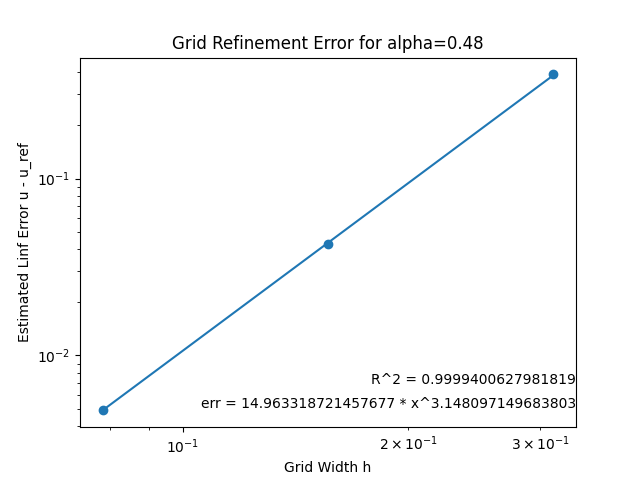
\includegraphics[width=\linewidth]{./error_plot_0.48.png}

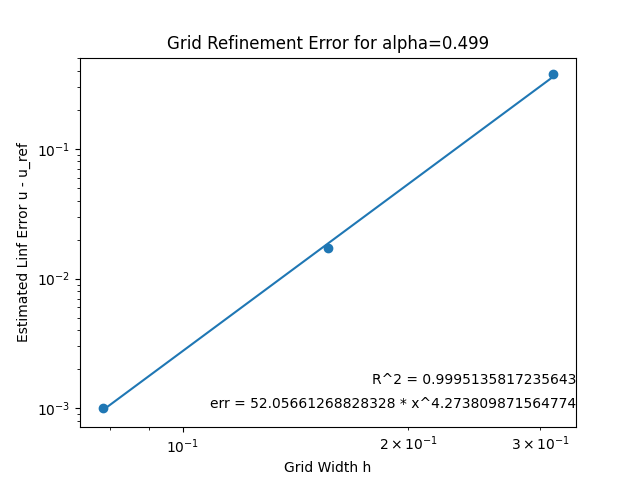
\includegraphics[width=\linewidth]{./error_plot_0.499.png}

\problemitem[3g)] Kelvin Helmholtz instability
\prob 

I think the plot is making 2 white for some reason? Not going to change it now though.

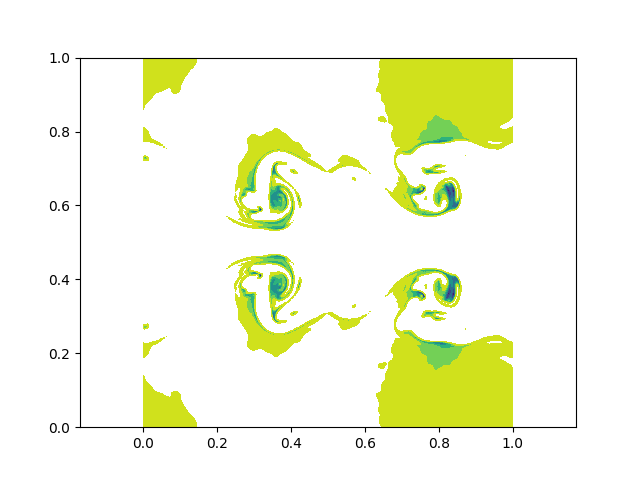
\includegraphics[width=\linewidth]{./helmholtz.png}
\end{problems}
\end{document}
% vim: set fdm=expr foldexpr=(getline(v\:lnum)=~'^\\s*\\\\item.*'?'a1'\:(getline(v\:lnum)=~'^\\s*\\\\begin.enumerate.*'?'a1'\:(getline(v\:lnum)=~'^\\s*\\\\end.enumerate.*'?'s2'\:(getline(v\:lnum+1)=~'^\\s*\\\\item.*'?'s1'\:(getline(v\:lnum)=~'^\\s*\\\\end.document.*'?0\:(getline(v\:lnum)=~'Begin\ My\ Stuff'?1\:(getline(v\:lnum)=~'End\ My\ Stuff'?'<1'\:'='))))))):
